\documentclass[12pt,a4paper]{report}
\usepackage[latin2]{inputenc}
\usepackage{graphicx}
\usepackage{ulem}
\usepackage{xcolor} 

\begin{document} 
\pagenumbering{roman}
\begin{center}
	\textbf{\Large{A Project Report}}
\end{center}

\begin{center}
	\textbf{on}
\end{center}

\begin{center}
	\textbf{ \Large{\textcolor{red}{ "Density based traffic light system"}}}
\end{center}

\begin{center}
	Submitted to the 
\end{center}

\begin{center}
	\large{Savitribai Phule Pune University} 
\end{center}

\begin{center}
	In partial fulfillment for the award of the Degree of
\end{center}

\begin{center}
	\large{Bachelor of Engineering} 
\end{center}

\begin{center}
	in
\end{center}

\begin{center}
	\large{Information Technology}
\end{center}

\begin{center}
	by
\end{center}

\begin{center}
	\textbf{\Large {Aditya Patil}}
\end{center}
\begin{center}
	\textbf{\Large {Bhushan Chandsare}}
\end{center}
\begin{center}
	\textbf{\Large {Omakr Ghadge}}
\end{center}
\begin{center}
	\textbf{\Large {Jayesh Kognole}}
\end{center}

\begin{center}
	Under the guidance of
\end{center}

\begin{center}
	\textbf{\Large{\textcolor{red}{Prof. Neha Rajas}}}
\end{center}





\begin{figure}[h]
\centering

\includegraphics[width=4cm,height=3cm]{stes.jpg}
\end{figure}

\begin{center}
	\textbf{\Large{\textcolor{red}{Department of Information Technology}}}
\end{center}

\begin{center} 
	\large {STES's Sinhgad College of Engineering}
\end{center}

\begin{center}
	Vadgaon (Bk.), Off. Sinhgad Road,
\end{center}

\begin{center}
	Pune 411041.\textbf{ }
\end{center}

\begin{center}
	\textbf{\Large{\textcolor{red}{Semester-VIII, Fourth Year Engineering}}}
\end{center}

\begin{center}
	\textbf{\large{2021-2022}}
\end{center}

%=====================================================================

\newpage

\begin{figure}[h]
\centering

\includegraphics[width=4cm,height=3cm]{stes.jpg}
\end{figure}

\begin{center}
	
	\textbf{\Large{CERTIFICATE}}
\end{center}
This is to certify that the project based seminar report entitled \textcolor{red}{"Density based traffic light system"} is
a record of bonafide work carried out by them under the supervision and guidance of Mrs. Jyoti Kulkarni in partial fulfillment of the requirement for \textcolor{red}{Prof.Neha Rajas} in partial fulfillment of the requirement for \textbf{BE (Information Technology Engineering) - 2015  Course} of Savitribai Phule Pune University, Pune in the academic year 2021-2022.\\
\\
Date:\ \ 
\\
\\Place:\ \ Pune
\\
\\\textcolor{blue}{Prof. Neha Rajas} \hspace{180pt} \textcolor{blue}{Prof. S. P. Potdar}
\\\hspace{20pt} Seminar Guide \hspace{180pt} Head of the Department
\\

 \begin{center}
 	\textcolor{blue}{Dr. S. D. Lokhande}\\
{Principal}
\end{center}

\noindent\rule{\textwidth}{0.4pt}
\par This Project Based Seminar report has been examined by us as per the Savitribai Phule Pune University, Pune requirements at STES's Sinhgad College of Engineering, Pune-411041 on . . . . . . . . . . .
\\
\\ \\Internal Examiner \hspace{180pt} External Examiner 
\begin{figure}[h]
	\centering
	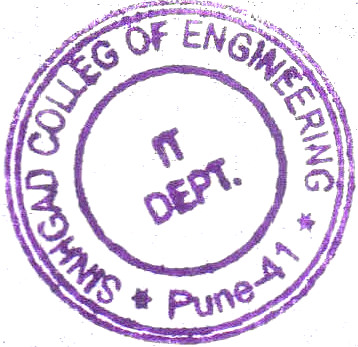
\includegraphics[width=2cm,height=2cm]{ITStamp.png}
\end{figure}


%======================================================================

\newpage

\begin{center}
	\textbf{\Large{ACKNOWLEDGMENT}}
\end{center}
I am highly indebted to my guide Prof. Neha Rajas for her guidance and constant supervision as well as for providing necessary information regarding the seminar report and also for his support in completing the seminar report. I would like to express my special gratitude and thanks
to Staff Members of department of Information Technology for giving me such attention and time.\par
This acknowledgment would be incomplete without expressing my thanks to Prof. S. P. Potdar, Head of the Department (Information Technology) for his support during the work.\par
I would like to extend my heartfelt gratitude to my Principal, Dr. S. D. Lokhande who provided a lot of valuable support, mostly being behind the veils of college bureaucracy.\par
I would also like to express my gratitude towards my parents and friends for their kind co-operation and encouragement which help me in completion of this report. My thanks and appreciations also go to my colleague in developing the seminar report and people who have willingly helped me out with their abilities.

\vspace{2cm}
Aditya Patil\par
Bhushan Chandsare\par
Jayesh Kognole\par
Omkar Ghadge\par

%========================================================================

\newpage

\begin{center}
	\textbf{\large {Abstract}}
\end{center}


Traffic is turning out to be one of the most increasing and serious problem for people worldwide and specially for countries like India .Due to increase in use of vehicles, the problem of congestion on roads is becoming a serious issue in cities .Four Indian cities including Bengaluru (1st rank )  , Mumbai (4th rank), Pune (5th rank ) ,  Delhi (8th rank) in 2019 among the top 10 most congested cities of the world. Bengaluru residents lose 243 hours on average (10 days and 3 hour) every year due to traffic.\par
This problem is not only limited to unwanted congestion in journey or triggering of stress in drivers but can be a serious threat to the environment too.About 27\% of air is polluted by vehicles.According to a report from European Environment Agency(EEA), outdoor air pollution could cause 6 to 9 million premature deaths a year by 2060. While there are a number of factors linked to this, a major contributor of pollutionis traffic, caused by the ever-increasing number of vehicles on the roads.
. With the use of Density Based Traffic control system the effect of traffic on air can be reduced significantly.\par


%========================================================================
\newpage
\begin{center}
	\textbf{\large {Contents}}
\end{center}

Certificate \hspace{235pt} 	ii

Acknowledgment \hspace{200pt} iii

Abstract \hspace{242pt} iv

Chapter Contents \hspace{195pt} vii

List of Figures \hspace{211pt} viii



\tableofcontents 
%========================================================================

\listoffigures
%========================================================================


%========================================================================
\newpage

\pagenumbering{arabic}

\chapter{\textbf{\Large{CHAPTER 1}}}
\section{\textbf{\large {Introduction to Project Topic}}}
\subsection{ Introduction to Project}
\begin{center}
	\textbf{\Large{Project Title  : Density based Traffic management system }}
\end{center}
	To minimize the traffic delays on the traffic signal.Traffic is turning out to be one of the most increasing and serious problem for people worldwide and specially for countries like India .Due to increase in use of vehicles, the problem of congestion on roads is becoming a serious issue in cities.\par
This increase in traffic leads to many problems such as increase in wait time.Due to ever increasing nature of traffic a density-based traffic control system is necessary that aids the swift movement of vehicles .This problem is not only limited to unwanted congestion in journey or triggering of stress in drivers but also serious threat to the environment. In this project we try to come up with a promising solution for the control of traffic.\par




\subsection{ Motivation behind project topic}

Due to increase in use of vehicles, the problem of congestion on roads is becoming a serious issue in cities .
Four Indian cities including Bengaluru (1st rank )  , Mumbai (4th rank), Pune (5th rank ) ,  Delhi (8th rank) in 2019 among the top 10 most congested cities of the world.
Bengaluru residents lose 243 hours on average (10 days and 3 hour) every year due to traffic. To put it in perspective an average Bengaluru resident could have watched 215 episodes of Game of Thrones or have done some productive work with the time spent while waiting on traffic signals .
About 27\% of air is polluted by vehicles.According to a report from European Environment Agency(EEA), outdoor air pollution could cause 6 to 9 million premature deaths a year by 2060. While there are a number of factors linked to this, a major contributor of pollutionis traffic, caused by the ever-increasing number of vehicles on the roads. 

\subsection{ Aim and Objective(s) of the work}

\textbf{Project aim:}
	 To minimize the time delays on the traffic signal and manage traffic effectively.
\ldots "
\\

\textbf{Project objectives:} 
	To increase the efficiency of traffic signals we intend to use 
	"Signal phase extension " and "Time adjustment theory".
\\
To compare the traditional traffic system with the Density Based Traffic system. 


\subsection{ Introduction to Seminar Topic}
This project  focuses to improve the efficiency of current traffic lights which will eventually redulce the waiting time of vehicle on traffic lights and eventually reduce the Environmental harms.We have achieved this using density based traffic control system which calculates the green signal time using the number of vehicles on that particular lane.
%=======================================================================

\begin{center}
	s
\chapter{\textbf{\Large{CHAPTER 2}}}
\end{center}

\section {\textbf{ Summary of Research Papers studied}}
	A New Approach for Intelligent Traffic Control System using Raspberry pi. ijirt,2017. An intelligent traffic control system is employed for a smooth flow of traffic. They used RFID for counting the number of vehicles to control the congestion by giving red signals.\par
5 th IEEE International Conference on Recent Advances and Innovations in Engineering- ICRAIE 2020: Smart Control of Traffic Light Using Artificial Intelligence: In this project Mr.Mihir and his team used image processing for traffic control and for the future modifications suggested a special service to the emergency vehicles.\par
IEEE (ICICCT 2018) :RFID-Based Smart Traffic Control Framework for Emergency Vehicles: In this proposed system arduino along with RFID is used which is very slow microcontroller  and can be replaced with better options.\par
Advanced Automation Control in an Ambulance under Emergency Condition(IEEE 2017): In this report the approach is using  RFID tags for scanning for ambulance but it does not tell the signal microcontroller in advance about the arrival.\par



\newpage		
\section{\textbf{Problems Identified}}
	
		
		\begin{figure}[h]
			\centering
			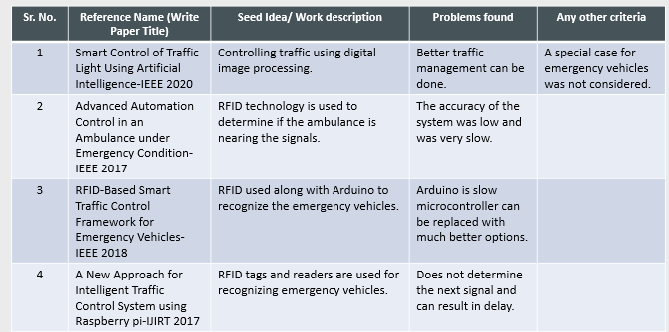
\includegraphics[width=150mm]{summary.png}
			\caption{Summary of literature survey}
			\label{fig_12}
		\end{figure}
				
	

%========================================================================

\begin{center}
	\chapter{\textbf{\Large{CHAPTER 3}}}
\end{center}
  
\section {\textbf{\large Density based traffic system}}
\subsection{ Introduction to Green signal timers}

We propose to calculate green signal timer by calculating the density of different class of vehicles on a particular lane of traffic signal junction ,this would have a rela time analysis and hence could help in smartly managing the traffic .

\subsection{Equations }
\begin{center}
\begin{math}
\bf\sum_n \frac{\huge t_n * \huge v}{\huge l}
\end{math}
\end{center}
where,\par
GST - Green signal timer\par
 n - class of vehicle \par 
t - average time for a class of vehicle to pass the junction\par
 v - count of vehicles of a patricular class\par
 c - capacity of sublane to hold vehicle of a particular class\par
 l - no of sublanes in a lane\par

\newpage
\subsection{Cases of Green Signal Time }
There can be three casses in Green Signal Time :\\ \par 

\textbf{case 1} - Calculated G.S.T. is less than minimum value . In that case the value of GST for that lane would be set to minimum value.\\ \par

\textbf{case 2 }-  Calculated G.S.T. is more than maximum value . In that case the value of GST for that lane would be set to maximum value.\\\ \par

\textbf{case 3} - Calculated G.S.T. is between maximum and minimum value . In that case the value of GST for that lane would be set to calculated value.\\ \par



\newpage
\section {\textbf{\large Vehicle classification}}


\subsection{ Types of vehicles}
\begin{tabular}{||l|c|r|p{6cm}||}
    Sr.No. & Class & Vehicle  \\
    1 & class 1 & Bus and Truck \\
    2 & class 2 &Tempo and Mini Bus \\
    3 & class 3 & 4-Wheeler cars \\
    4 & class 4 & Rikshaw and other 3-Wheelers \\
    5 & class 5 & Bikes and other 2-Wheelers \\
\end{tabular}
\subsection{Classification Method }
The video of lane is captured by the cameras instaled on every signal and number of vehicles are calculated through openCV and YOLO v5
(In our project we have selected a video from local computer which acts as the captured video).            
\newpage
       
\section {\textbf{\large YOLO v5 }}
\subsection{ Intorduction}
CNN-based Object Detectors are primarily applicable for recommendation systems. YOLO (You Only Look Once) models are used for Object detection with high performance. YOLO divides an image into a grid system, and each grid detects objects within itself. They can be used for real-time object detection based on the data streams. They require very few computational resources.

\subsection{Why IoT }
{\textbf Automation and Control}
Due to physical objects getting connected and controlled digitally and centrally with wireless infrastructure, there is a large amount of automation and control in the workings Without human intervention, the machines are able to communicate with each other leading to faster and timely output.\par
{\textbf Cost Efficientl}
The biggest advantage of IoT is saving money. If the price of the tagging and monitoring equipment is less than the amount of money saved, then the Internet of Things will be very widely adopted. IoT fundamentally proves to be very helpful to people in their daily routines by making the appliances communicate to each other in an effective manner thereby saving and conserving energy and cost. Allowing the data to be communicated and shared between devices and then translating it into our required way, it makes our systems efficient.\par
{\textbf Fast and Efficientl}
The machine-to-machine interaction provides better efficiency, hence; accurate results can be obtained fast. This results in saving valuable time. Instead of repeating the same tasks every day, it enables people to do other creative jobs.\par
{\textbf Information}
It is obvious that having more information helps making better decisions. Whether it is mundane decisions as needing to know what to buy at the grocery store or if your company has enough widgets and supplies, knowledge is power and more knowledge is better.
\newpage   
\section {\textbf{\large Implementation}}
\subsection{ IoT using Cloud}
IoT devices can generate lots of data, cloud computing paves the way for this data to travel\par
Cloud computing enables the storage and analysis of data to be done quickly and I n real-time\par
IoT cloud platform: IoT device has multiple sensors and it is connected to the cloud via gateways. Eg. AWS IoT, Microsoft Azure IoT Hub, Google Cloud IoT, IBM Watson IoT Platform\par
\newpage     
\subsection{ RFID Implementation}
RFID is used in this system to detect the emergency vehicles which are nearing the signal which has a RFID reader installed in it which connects to a microcontroller and communicates with the cloud to send signal when emergency vehicles come near to the signal.
\par      

    
   \begin{figure}[h]
			\centering
			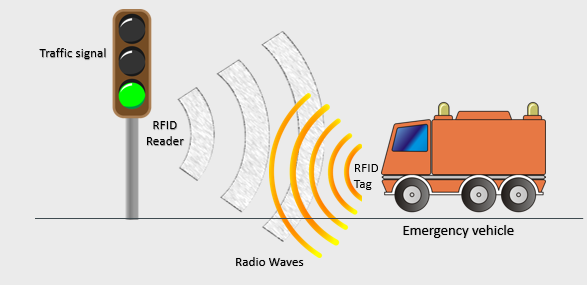
\includegraphics[width=150mm]{impkrfid.png}
			\caption{RFID Implementation}
			\label{fig_23}
		\end{figure}
\newpage   
\subsection{Actual Implementation}
Step1: Scan the lane using OpenCV through cameras and classify the vehicles using YOLOv5.\par
Step2: Through the number of different types of vehicles in that lane calculate the Green Signal Time using the formula.\par
Step3: From the given casses decide time that must be allocated to that lane. \par
Step4: Assign the Green Signal Time for the particular signal\par
Step5: Scan the next lane\par    


%========================================================================

\begin{center}
	\chapter{\textbf{\Large{CHAPTER 4}}}
\end{center}
  
\section{\textbf{Conclusions}}
In this seminar we studied about Inter net of things, cloud computing, RFID technology and how we are going to use it for swift movement of vehicles.\par
Using these techniques together is going to assist the movement of emergency vehicles and will surely help in saving people's life.\par
 The topics discussed in this seminar are one of the most important domains we will implement in our project.  \par

%========================================================================

\newpage

\section{\textbf{References}}

List all the material used from various sources for making this project proposals

\begin{enumerate}
\item Smart Control of Traffic Light Using Artificial Intelligence-IEEE 2020- (Mihir M. Gandhi Dept. of Computer Engineering K.J. Somaiya College of Engineering, Vidyavihar ).

\item Advanced Automation Control in an Ambulance under Emergency Condition-IEEE 2017- (Lella Sai Krishna1 UG Student EEE Department Sathyabama University Chennai).

\item RFID-Based Smart Traffic Control Framework for Emergency Vehicles-IEEE 2018- (Tejas Naik, Roopalakshmi R, Divya Ravi N, Pawdhan Jain, Sowmya B H and Manichandra).

\item A New Approach for Intelligent Traffic Control System using Raspberry pi-IJIRT 2017- (P. Nandini Kiran1 1M.Tech student, Dept. of ECE,CMR Technical Campus,Hyderabad, Telangana, India).


\end{enumerate}

\end{document}
